\documentclass[a4paper,12pt]{article}

\usepackage{geometry}       % Required for page layout.
\usepackage{hyperref}       % Required for hyperlinks.
\usepackage{graphicx}       % Required for figures.
\usepackage{subfig}         % Required for minipages.
% \usepackage{caption}
% \usepackage{subcaption}
\usepackage{placeins}
\usepackage{float}

\newgeometry{vmargin={25.4mm}, hmargin={27mm,27mm}}
\setlength\parindent{0pt}   % Disable paragraph indent.

\title{Project 2: Random Processes and Complex Systems}
\author{
  Elias Rilegård\\
  \texttt{eliasril@kth.se}
}

\begin{document}
\maketitle

\section*{Exercise 2.1: Polymers as 2D Random Walks}

This exercise revolves around organic polymers and ways to approximate and simulate them using mathematical random
walks.

\subsection*{Part a}

The task was to write a program that generates a 2D random walk with single steps along the x or y axis, and then
to generate random walks of length $10$, $100$, and $1000$. Shown below are samples of the walks generated.

\begin{figure}[!ht]
  \centering
  \begin{minipage}{0.45\textwidth}
    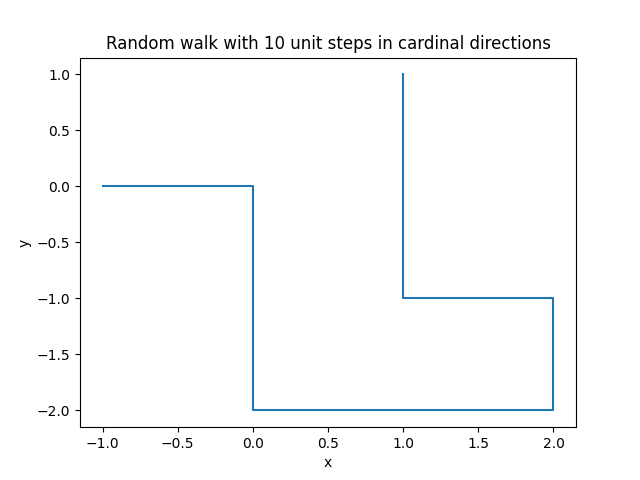
\includegraphics[width=\textwidth]{img/2_1a_random_10.png}
  \end{minipage}
  \begin{minipage}{0.45\textwidth}
    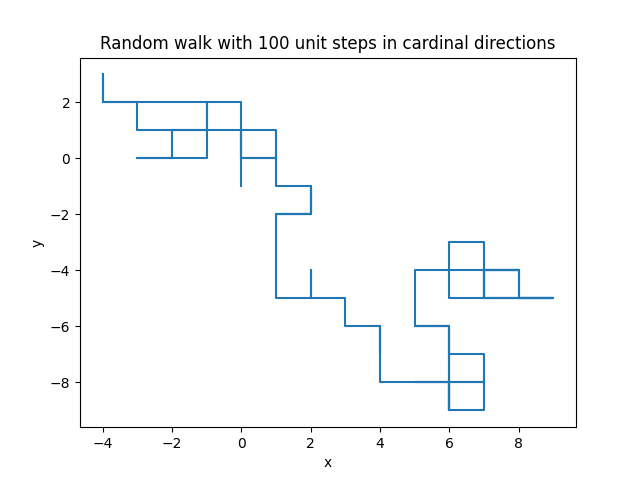
\includegraphics[width=\textwidth]{img/2_1a_random_100.png}
  \end{minipage}
  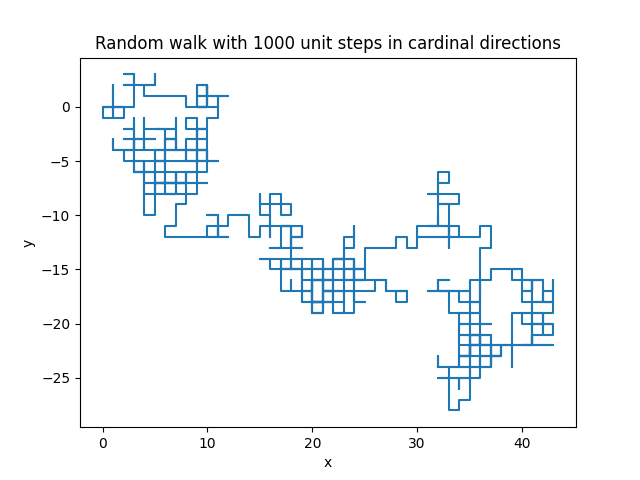
\includegraphics[scale=0.45]{img/2_1a_random_1000.png}
\end{figure}

\subsection*{Part b}

Instead of using Python's \texttt{random} library and its \texttt{random()} method, we instead use a pseudo-random
number generator defined by $r_n = (a r_{n - 1} + c)\, \%\, m$. Generating random walks of length $1000$ using the

Using the given parameters of $r_0 = 1$, $a = 3$,
$c = 4$, $m = 128$ and then $m = 129$, generating random walks of length $1000$ yields the following:

\begin{figure}[!ht]
  \centering
  \begin{minipage}{0.48\textwidth}
    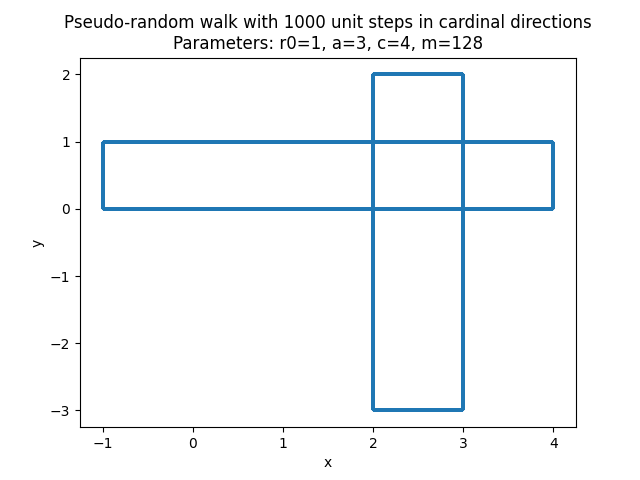
\includegraphics[width=\textwidth]{img/2_1b_pseudo_m128.png}
  \end{minipage}
  \begin{minipage}{0.48\textwidth}
    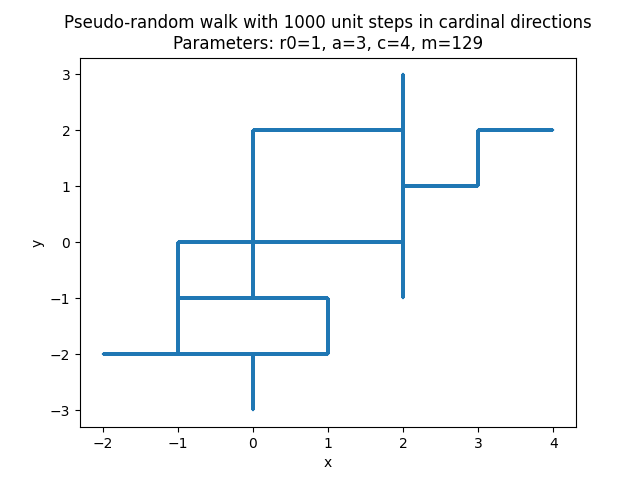
\includegraphics[width=\textwidth]{img/2_1b_pseudo_m129.png}
  \end{minipage}
\end{figure}

It's quite obvious that for these parameters, the random number generator has a very small period. Trying completely
random parameters yielded some... interesting results to say the least:

\begin{figure}[!ht]
  \centering
  \begin{minipage}{0.48\textwidth}
    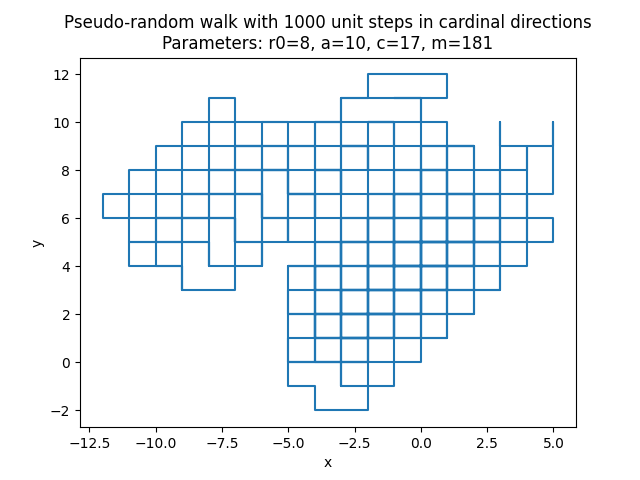
\includegraphics[width=\textwidth]{img/2_1b_free_grid.png}
  \end{minipage}
  \begin{minipage}{0.48\textwidth}
    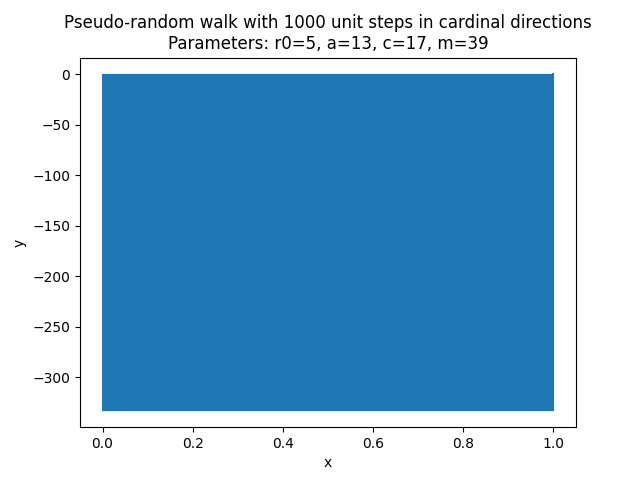
\includegraphics[width=\textwidth]{img/2_1b_free_filled.png}
  \end{minipage}
  \begin{minipage}{0.48\textwidth}
    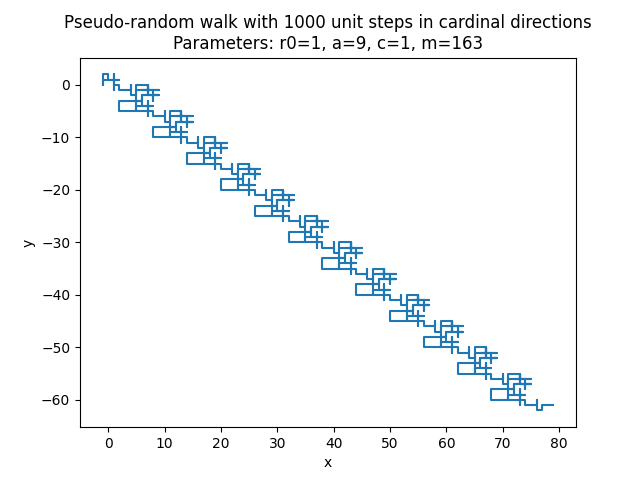
\includegraphics[width=\textwidth]{img/2_1b_free_links.png}
  \end{minipage}
  \begin{minipage}{0.48\textwidth}
    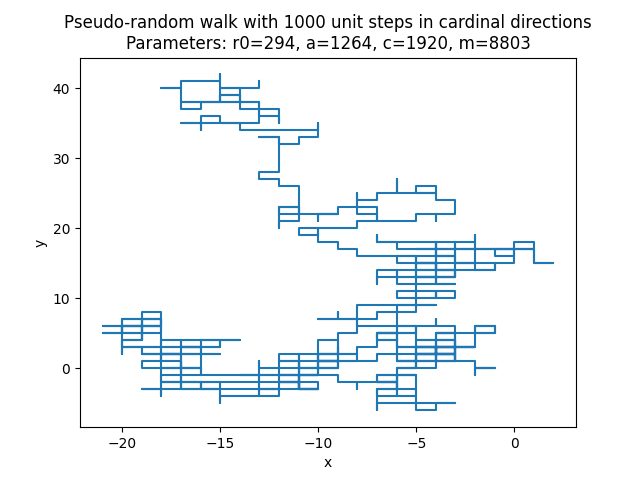
\includegraphics[width=\textwidth]{img/2_1b_free_big2.png}
  \end{minipage}
\end{figure}

Do note the wildly different scales on the axes, which partially explains some of the behavior. For some sets of
parameters, the walk displays a clear pattern and period, while for other sets the period time is much greater,
resulting in what appears to be "better" randomness.

\subsection*{Part c}

Generating many random walks for a few (but not necessarily all 100) values of the step number in the range from
$1$ to $1000$, we want to determine the root mean squared end-to-end distance (henceforth abbreviated as RMSD)
$\sqrt{<\!R^{2}\!>}$ and the root-mean-square fluctuation (RMSF) $\sqrt{(<\!R^2\!>\!-\, {<\!R\!>}^2) \frac{M}{M - 1}}$,
where $M$ is the number of samples. With $R^2 = x^2 + y^2$, we can visualize the quantities and their dependence
on $N$ as

\begin{figure}[!ht]
  \centering
  \begin{minipage}{0.48\textwidth}
    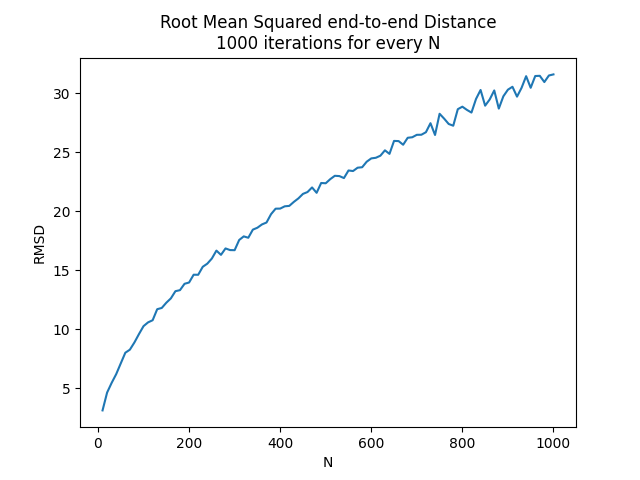
\includegraphics[width=\textwidth]{img/2_1c_rmsd_1000.png}
  \end{minipage}
  \begin{minipage}{0.48\textwidth}
    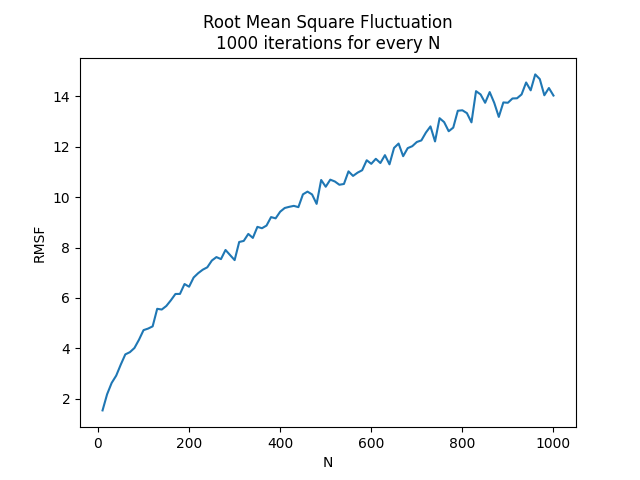
\includegraphics[width=\textwidth]{img/2_1c_rmsf_1000.png}
  \end{minipage}
\end{figure}

We can also caculate the standard error estimate as $\sqrt{\frac{<\!R^2\!> - {<\!R\!>}^2}{M - 1}}$, which is also
dependant on $N$:

\begin{figure}[!ht]
  \centering
  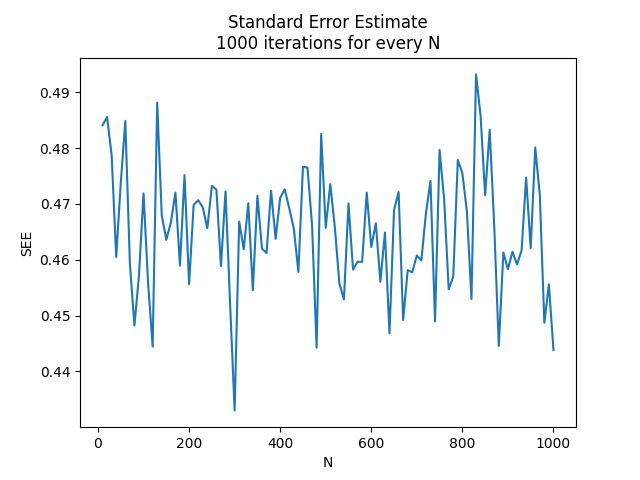
\includegraphics[scale=0.48]{img/2_1c_stderrest_1000.png}
\end{figure}

While the standard error estimate looks chatotic, it's actually contained in a small range, and perhaps more
importantly, is more or less constant for all $N$.

\subsection*{Part d}

A real polymer can not cross itself, since different atoms can't occupy the same space. We can better simulate this
by crafting a self avoiding random walk. In order to ensure the randomness of the walk, any walk which lands on a
coordinate pair it's already visited will be discarded. We can slightly improve this algorithm by restricting the
walk to immediately turn back on itself, i.e. it can only continue forward, turn right or turn left (relative to the
direction it came from). Of course, generating walks and discarding it as soon as it steps on to itself means the
success rate (that is, the fraction of walks that finishes generating without stepping on itself) will decrease as
the length of the walk increases. This relation is visualized in the following graphs:

\begin{figure}[!ht]
  \centering
  \begin{minipage}{0.48\textwidth}
    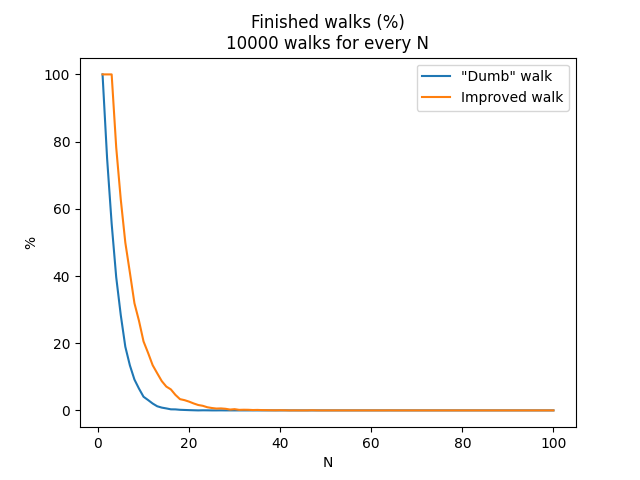
\includegraphics[width=\textwidth]{img/2_1d_percent_completed_comparison_10000.png}
  \end{minipage}
  \begin{minipage}{0.48\textwidth}
    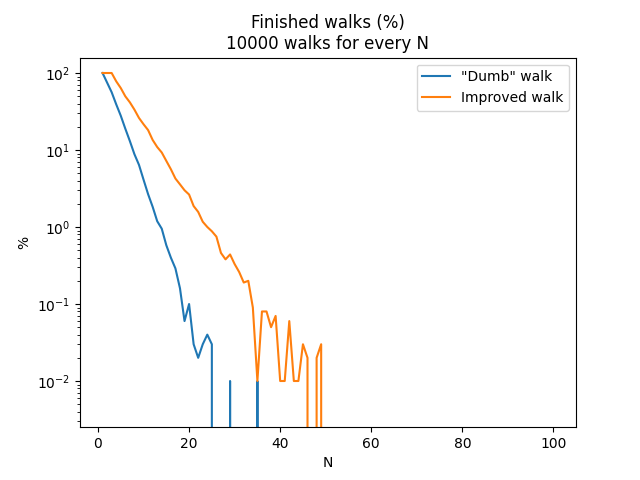
\includegraphics[width=\textwidth]{img/2_1d_percent_completed_comparison_log_10000.png}
  \end{minipage}
\end{figure}

As is expected, the improved walk performs marginally better than its "dumb" counterpart. To determine the maximum
value of $N$ that one can reasonably consider, we first have to note that it will slightly differ from computer to
computer, depening on its processing power and how much one is willing to brute force. However, on the machine I am
running the simulations on, together with an arbitrary success rate limit of $0.1\%$, a value of $N \approx 35$ seems
somewhat adequate.

\subsection*{Part e}

Computing the RMSD (end-to-end) for the improved self avoiding walk in the range $N \in [1, 35]$ yields the following:

\begin{figure}[!ht]
  \centering
  \begin{minipage}{0.48\textwidth}
    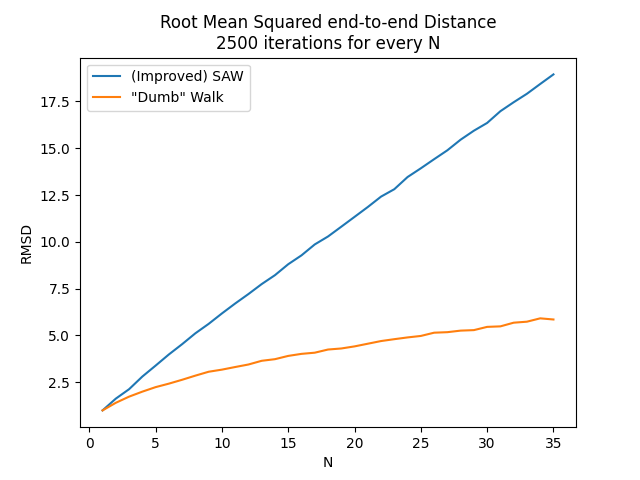
\includegraphics[width=\textwidth]{img/2_1e_rmsd_2500.png}
  \end{minipage}
  \begin{minipage}{0.48\textwidth}
    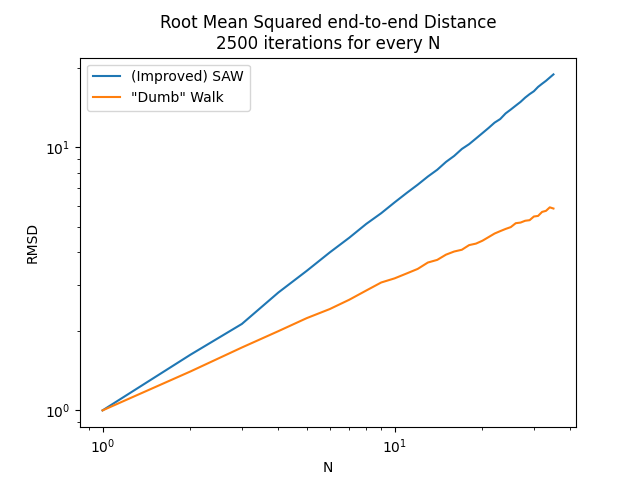
\includegraphics[width=\textwidth]{img/2_1e_rmsd_loglog_2500.png}
  \end{minipage}
\end{figure}

Compared to a normal "dumb" random walk, the RMSD for a self avoiding walk seems to have a linear correlation with
its length. For reference, the correlation for the "dumb" walk appears to be $\propto \sqrt{N}$, due to the shape
of the normal plot being roughly square root shaped, and the slope in the loglog plot being approximately
$\frac{1}{2}$.

\pagebreak

\section*{Exercise 2.2: Traffic Model using Cellular Automata}

This exercise comprises of simulating car traffic using a cellular automaton model.

\subsection*{Part a}

Implementing the cellular automaton traffic model \emph{with periodic boundary conditions} and running the simulation
using the parameters $v_{max} = 2$ and $p = 0.5$, for different car densities $\rho$ (defined by number of cars
divided by the road length) and computing the average flow rate nets the following fundamental diagram.

\begin{figure}[!ht]
  \centering
  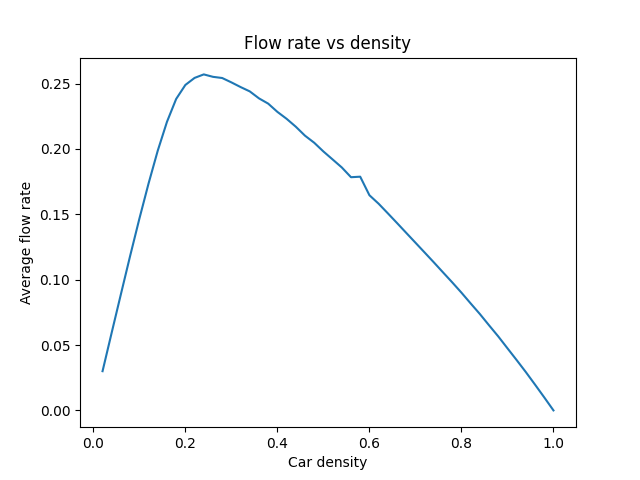
\includegraphics[scale=0.48]{img/2_2a_fr_density.png}
\end{figure}

The flow rate peaks in this graph at $\rho = 0.24$ with a flow rate of $0.255$. As the number of cars increases,
they're at first not restricted by each other (in regards to having to break or keep a lower maximum velocity). This
means they can all run at their highest velocity, meaning adding more cars increases the car throughput without any
hindrance, even considering the random breaks some cars do. At $\rho = 0.24$ though, this changes. Now there are
enough cars per unit of road that some will have to deliberately start braking to not crash into the car in front
of it. Thus, all cars will on average have a lower speed, meaning the flow rate will also be lower. Further increasing
the number of cars amplifies this effect, with all cars having to drive with an even lower average speed. This effect
continues all the way up until $\rho = 1$, where we arrive at a complete traffic jam. Now no car can move at all
without crashing into the car in front of it.

\subsection*{Part b}

This part is all about computing the statistical accuracy. Using a road length of 50, 25 cars, $v_{max} = 2$ and
$p = 0.5$, multiple simulations were run, collecting the flow rate averaged over 100 time steps. From this, it's
possible to then calculate the standard error of the flow rate, using the same formula as listed in Section 2.1c.
The following graph describes the dependance of the standard error estimate (SEE) as a function of the number of
simulations done.

\begin{figure}[!ht]
  \centering
  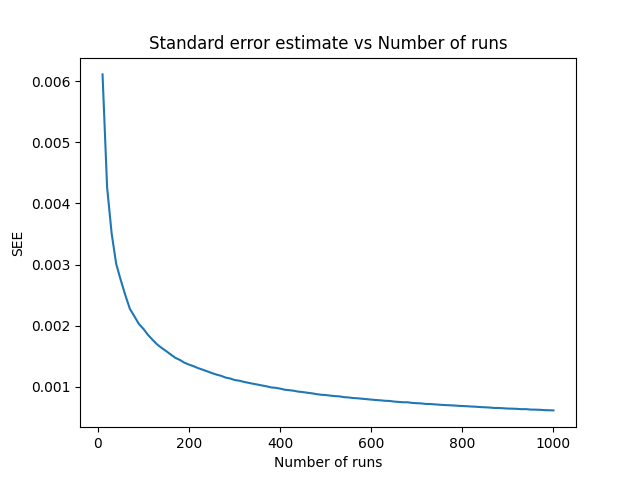
\includegraphics[scale=0.48]{img/2_2b_SEE.png}
\end{figure}

\FloatBarrier

To achieve a standard error of $0.001$, about 380 simulations needs to be performed. It's clear from the graph that
going any lower with the standard error results in highly diminishing returns.
To answer the question regarding how long the equilibration time needs to be before accurate results show up,
consider the following graph where the average flow rate has been drawn versus the number of steps in the simulation.

\begin{figure}[!ht]
  \centering
  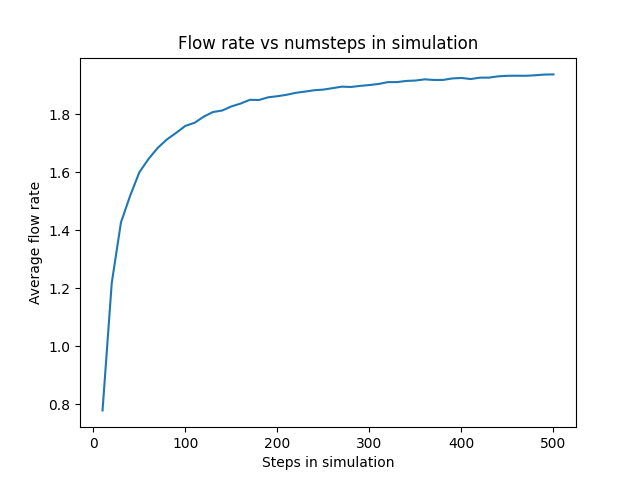
\includegraphics[scale=0.48]{img/2_2b_flowrate_nsteps.png}
\end{figure}

Here, \emph{all} flow rates from the entire simulation has been recorded instead of only sampling when the simulation
has more or less entered a state of equilibrium. It quickly becomes apparent that a step count of anything under $100$
will yield very sqewed results, at least when sampling the flow rate over every timestep. Approaching $100$ (or even
better, $200$) time steps, we notice that the curve starts to flatten out, since the settling period of the system now
only comprises a relatively small portion of the total running time. We can therefore draw a conclusion that any
time step count below $100$ will \emph{not} yield accurate results.

\subsection*{Part c}

To determine when the fundamental diagram becomes independent of the size of the system (i.e. the length of the road
has no effect on the results), the simulation to generate the fundamental diagram was run multiple times for each
length of the road. This yielded the following graph:

\begin{figure}
  \centering
  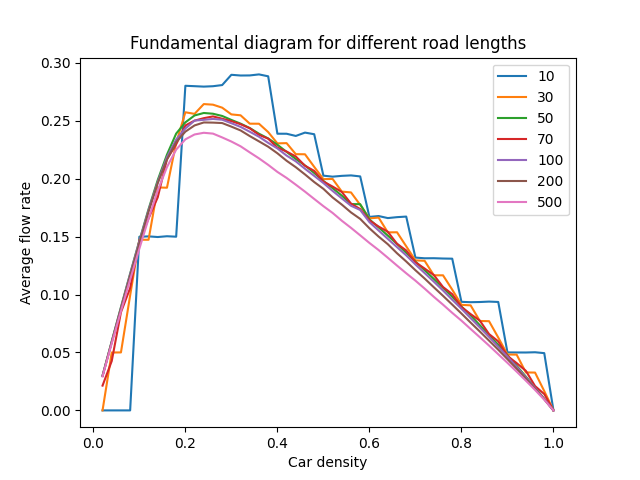
\includegraphics[scale=0.48]{img/2_2c_flowrate_density.png} % Ev ta bort 500?
\end{figure}

\FloatBarrier

It's quite obvious that the system looks self-similar for most values of the road length, however at very low values
($10$ and partially $30$), the graph is still jagged, which is mainly caused by the number of cars being rounded to
an integer during testing, but also the impact of a single car braking being comparably higher. Either way, the
fundamental diagram starts looking self-similar at a road length of 50 and above.

\subsection*{Part d}

% Part d and e mainly revolves around altering $v_{max}$ and $p$, the probability of a car randomly slowing down.
Generating the system's fundamental diagram for different values of $v_{max}$ yields the following graph on the left:

\begin{figure}[!ht]
  \centering
  \begin{minipage}{0.48\textwidth}
    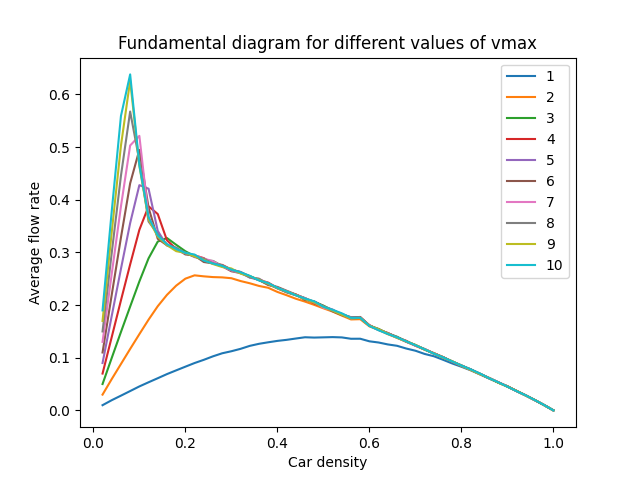
\includegraphics[width=\textwidth]{img/2_2d_fundamental.png}
  \end{minipage}
  \begin{minipage}{0.48\textwidth}
    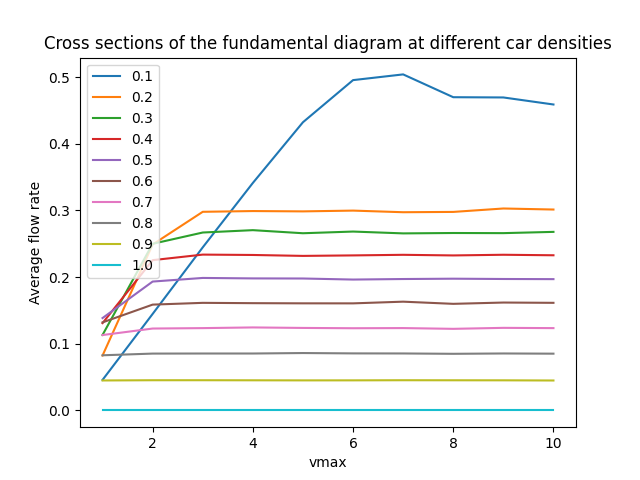
\includegraphics[width=\textwidth]{img/2_2d_flowrate_vmax_2.png}
  \end{minipage}
\end{figure}

The graph on the right shows a cross section of the graph on the left at different values of the car density $\rho$.
It's rather self-explanatory that a higher maximum speed leaves potential for a higher average flow rate, but the
graph makes it really obvious. With $v_{max} = 1$, until the car density $\rho$ reaches $0.5$, the road always has
capacity for a higher car throughput. As $\rho$ increases beyond $0.5$, the cars start having to slow down due to
approaching the car that's in front of it, lowering the average flow rate. This phenomenon also shows up as $v_{max}$
increases, however the threshold for maximum average flow rate occurs much earlier, with the actual maximum average
flow rate (the peak of each curve) increasing akin to some function $f(x) = \frac{1}{x}$.

\subsection*{Part e}

This part is almost identical to Part d except now we're varying $p$, the probability of a car randomly braking at
any point. Generating the fundamental diagram for the system for different values of $p$ here yields the following
graph on the left:

\begin{figure}[!ht]
  \centering
  \begin{minipage}{0.48\textwidth}
    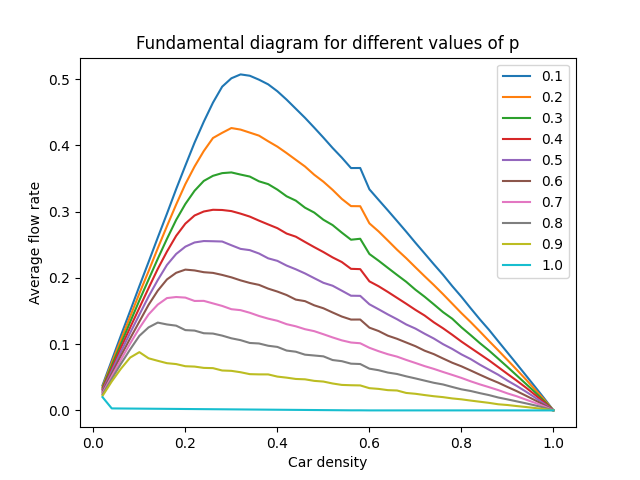
\includegraphics[width=\textwidth]{img/2_2e_fundamental.png}
  \end{minipage}
  \begin{minipage}{0.48\textwidth}
    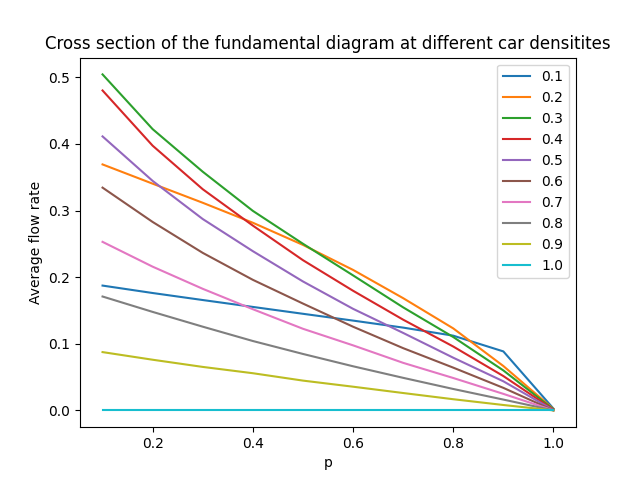
\includegraphics[width=\textwidth]{img/2_2e_flowrate_p_2.png}
  \end{minipage}
\end{figure}

Again, the graph on the right shows a cross section of the graph on the left at different values of the car density
$\rho$. We note that someting close to the same phenomenon appearing here, in regards to there being some sort of
"invisible" curve that the peaks of every graph follows. What's interesting to note is that when $p = 1$, there can
only be a single car on the road before the total car flow becomes zero. As $p$ decreases, the maximum average flow
rate increases as well, moving slightly to the right on the graph. This is due to the chance of congestion decreasing,
allowing more cars to travel at higher speeds, even at higher values of $\rho$.

\end{document}